
\section{Theorie}
\label{sec:Theorie}
\subsection{Wärmekapazität}
\label{sec:Wärmekapazität}
Die Wärmekapazität $C$ beschreibt die Energie, die benötigt wird um 1 Mol eines Stoffes um 1 Kelvin zu erhitzen und ist definiert als:
\begin{equation}
  \label{eqn:Wärmekapazität}
  C=\dfrac{\Delta Q}{\Delta T}
\end{equation}
Dabei müssen die Randbedingungen betrachtet werden. Dabei wird unterschieden zwischen der Temperaturänderung bei konstantem Druck oder bei konstantem Volumen. Das folgende Experiment wird bei konstantem Druck durchgeführt, da für das Gewährleisten eines konstanten Volumens bei der thermischen Ausdehnung ein sehr hoher Druck benötigt würde. Die Berechnung der Wärmekapazität bei konstantem Druck $C_\mathrm{p}$ erfolgt mit einem Korrekturfaktor:
\begin{align}
  \label{eqn:cv}
 C_\mathrm{V} = C_\mathrm{p}-9\alpha^2\kappa V_\mathrm{0}T
\end{align}
Dabei ist $\alpha$ ein Korrekturfaktor der aus der Anleitung entnommen werden kann \cite[3]{Anleitung}, $\kappa$ das Kompressionsmodul und $V_\mathrm{0}$ das molare Volumen.
Auch kann die Debye-Temperatur $\Theta_\mathrm{D}$ bestimmt werden. Die Debye-Temperatur ist eine materialspezifische Größe und bezeichnet die Temperatur bei der alle Zustände besetzt sind.
Im Folgenden werden drei Theorien beschrieben:
\subsection{Klassische Theorie}
\label{sec:Klasische Theorie}
Die klassische Betrachtung der Wärmekapazität besagt, dass die thermische Energie eines Körpers auf alle drei Freiheitsgrade der Atome gleichmäßig verteilt wird. Die Atome führen um ihre Ruhelage harmonische Schwingungen aus. Die kinetische Energie dieser Schwingungen ist gleich der thermischen Energie und beträgt pro Freiheitsgrad $\dfrac{1}{2}k_\mathrm{B}T$. Die kinetische Energie ist die Summe der drei Freiheitsgrade und beträgt deshalb:
\begin{align}
  \label{eqn:klassische Energie}
 E_\mathrm{kin} = \dfrac{3}{2}k_\mathrm{B}T
\end{align}
Dabei ist $k_\mathrm{B}$ die Boltzmann-Konstante. Mit der Loschmidt-Konstante $N_\mathrm{L}$, die die Teilchendichte eines idealen Gases beschreibt, ergibt sich in einem Kristall die Energie zu:
\begin{align}
  \label{eqn:Energie im Kristallk}
 E_\mathrm{kin} = \dfrac{3}{2}k_\mathrm{B}N_\mathrm{L}T
\end{align}
Weiter gilt $E_\mathrm{kin}=E_\mathrm{pot}$, daher ergibt sich für die Gesamtenergie $E_\mathrm{ges}$:
\begin{align*}
  E_\mathrm{ges}&= E_\mathrm{kin}+E_\mathrm{pot} \\
  E_\mathrm{ges}&= 3 k_\mathrm{B}N_\mathrm{L}T
\end{align*}
Bei konstantem Volumen folgt für die spezifische Wärmekapazität:
\begin{align}
  \label{eqn:3R}
 C_\mathrm{V} = 3R
\end{align}
Die spezifische Wärmekapazität ist somit in der klassischen Theorie nicht materialabhängig. In Experimenten zeigen sich Abweichungen: Zum einen ist die spezifische Wärmekapazität materialabhängig und zweitens zeigt sich die Annahme nur bei hohen Temperaturen. Darum muss die klassische Theorie als unzureichend angenommen werden.
\subsection{Einstein-Theorie}
\label{sec:Einstein-Theorie}
Die Annahmen des Einstein’schen-Modells besagen, dass alle Atome mit derselben Frequenz schwingen, aber deren Schwingungen gequantelt sind. Die Boltzmann'sche Wahrscheinlichkeitsverteilung
\begin{align}
  \label{eqn:Boltzmann}
 W(E) = \exp\left(\dfrac{-n \hbar\omega_\mathrm{E}}{k_\mathrm{B}T}\right)
\end{align}
beschreibt die Wahrscheinlichkeit des Antreffens eines Atoms im Zustand mit der Energie $n \hbar\omega_\mathrm{E}$ bei der Temperatur $T$. Durch das Aufsummieren der Wahrscheinlichkeitsverteilung ergibt sich die Einstein-Energie:
\begin{align}
  \label{eqn:Einstein-Energie}
 E_\mathrm{Einstein} = \dfrac{\hbar\omega_\mathrm{E}}{\exp\left(\dfrac{\hbar\omega_\mathrm{E}}{k_\mathrm{B}T}\right)-1}
\end{align}
Daraus folgt für die Wärmekapazität:
\begin{align}
  \label{eqn:Einstein Wärmekapazität}
 C_\mathrm{V} = 3R \left(\dfrac{\hbar\omega_\mathrm{E}}{k_\mathrm{B}T}\right)^2 \dfrac{1}{T^2} \dfrac{\exp\left(\dfrac{\hbar\omega_\mathrm{E}}{k_\mathrm{B}T}\right)}{\left(\exp\left(\dfrac{\hbar\omega_\mathrm{E}}{k_\mathrm{B}T}\right)-1\right)^2}
\end{align}
Dabei ist $\dfrac{\hbar\omega_\mathrm{E}}{k_\mathrm{B}T}$ die Einstein-Temperatur. Bei dem Einstein-Modell zeigt sich das Verhältnis von $ C_\mathrm{V} \approx 3R$ bei sehr hohen Temperaturen. Für tiefe Temperaturen nimmt  $C_\mathrm{V}$ exponentiell zu. Aber auch hier zeigen sich Abweichungen von experimentellen Werten.
\subsection{Debye-Modell}
\label{sec:Debby-Modell}
Das Debye-Modell basiert auf einer unterschiedlicher Frequenzverteilung $Z(\omega)$ mit einer Grenzfrequenz $\omega_\mathrm{D}$. Durch die nur drei Dimensionen besitzt ein Kristall nur 3 $N_\mathrm{L}$ Eigenschwingungen. Die Debye-Frequenz kann deshalb für hohe Temperaturen über
\begin{align}
  \label{eqn:Deby-Frequenz}
 \int_{0}^{\omega_\mathrm{D}} Z(\omega) \mathrm{d}\omega = 3N_\mathrm{L}
\end{align}
berechnet werden. Durch die Verknüpfung von klassischem und quantenmechanischem Modell ergibt sich für die Dichte der Eigenschwingungen:
\begin{align}
  \label{eqn:Eigenschwingungen2}
 Z(\omega) \mathrm{d}\omega = \dfrac{L^3}{2\pi^2} \omega^2 \left(\dfrac{1}{v_\mathrm{long}^3}+\dfrac{2}{v_\mathrm{trans}^3}\right) \mathrm{d}\omega
\end{align}
Dabei ist $L$ die Länge des Kristalls, $v_\mathrm{long}$ die Schallgeschwindigkeit in longitudinaler Ausbreitungsrichtung und $v_\mathrm{trans}$ die Schallgeschwindigkeit in transversaler Ausbreitungsrichtung.
Weiter wird angenommen, dass Frequenz und Ausbreitungsrichtung keine Auswirkungen auf die Phasengeschwindigkeit haben.
Die Debye-Frequenz kann wie folgt angegeben werden:
\begin{equation}
  \label{eqn:Eigenschwingungen}
  \omega_\mathrm{D}^3=\dfrac{18\pi^2N_\mathrm{L}}{L^3}\dfrac{v_\mathrm{long}^3v_\mathrm{trans}^3}{v_\mathrm{trans}^3+2v_\mathrm{long}^3}
\end{equation}
Mit der Debye-Grenzfrequenz ergibt sich:
\begin{align}
  \label{eqn:Debby 3}
 Z(\omega) \mathrm{d}\omega = \dfrac{9N_\mathrm{L}}{\omega_\mathrm{D}^3} \omega^2 \mathrm{d}\omega
\end{align}
Zur Ermittlung der Energie wird das Integral über alle Schwingungsmodi gebildet und durch die mittlere Energie einer Gitterschwingung geteilt, wodurch die Energie sich zu
\begin{align}
  \label{eqn:Debye-Energie}
 U = \int_{0}^{\omega_\mathrm{D}} \dfrac{Z(\omega) \mathrm{d}\omega}{\exp\left(\dfrac{\hbar\omega}{k_\mathrm{B}T}\right)-1}
\end{align}
und die Wärmekapazität $C_\mathrm{V,Debye}$ nach der Berechnung des Integrals zu
\begin{align}
  \label{eqn:DebyeWärmekapazität}
 C_\mathrm{V,Debye} = \dfrac{\mathrm{d}}{\mathrm{d}T}  \dfrac{\hbar 9N_\mathrm{L}}{\omega_\mathrm{D}^3} \int_{0}^{\omega_\mathrm{D}} \dfrac{\omega^3}{\exp\left(\dfrac{\hbar\omega}{k_\mathrm{B}T}\right)-1}
\end{align}
Für niedrige Temperaturen nähert sich das Debye-Modell einem $T^3$ Verlauf an, für hohe Temperaturen ist es ebenfalls annähernd $3R$.
\subsection{Vergleich der Modelle}
\label{sec:Vergleich der Modelle}
Bei einem Vergleich der drei Modelle zeigt sich, dass alle drei sich bei hohen Temperaturen ($T>\SI{300}{\kelvin}$) dem Wert $3R$ annähern. In tiefen Temperauren steigt die Wärmekapazität beim Einstein-Modell exponentiell und beim Debye-Modell mit $T^3$. Das freie Elektronengas hat eine lineare Abhängigkeit, dessen Auswirkungen nur bei tiefen Temperaturen ($T \rightarrow 0$) relevant sind. Am nähesten beschreibt dabei das Debye-Modell den experimentellen Verlauf. In Abbildung (\ref{fig:tkurve}) sind die drei Modelle schematisch dargestellt.
\begin{figure}
	\centering
	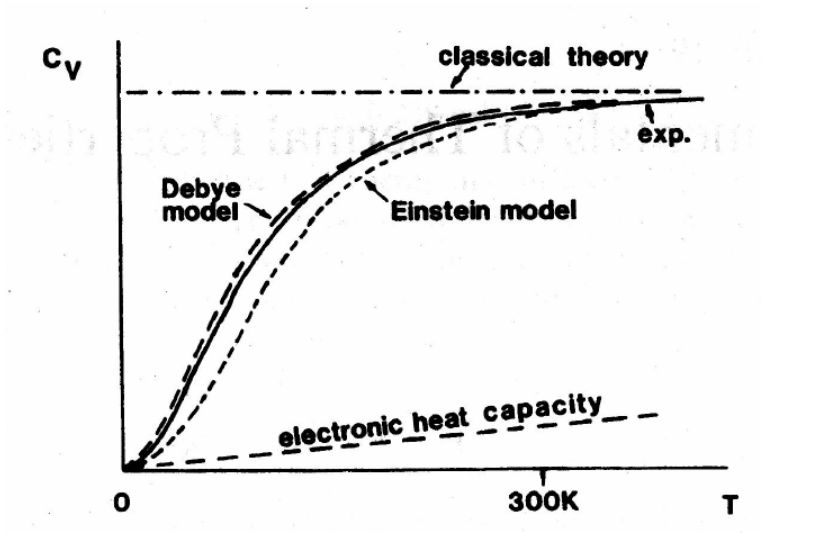
\includegraphics[scale=0.5]{fig/tkurve.png}
	\caption{Vergleich der drei theoretischen Modelle für den Verlauf der Wärmekapazität in Abhängigkeit von der Temperatur \cite{Anleitung10}.}
	\label{fig:tkurve}
\end{figure}
\FloatBarrier
